\documentclass[utf8,german,beleg]{zihpub}

\usepackage{datetime}
\usepackage{etoolbox}
\usepackage[acronyms,nomain,nonumberlist,xindy]{glossaries}
\usepackage[section]{minted}
\usepackage{tcolorbox}
\usepackage{tikz}
\usepackage{tikz-3dplot}

\BeforeBeginEnvironment{minted}{\begin{tcolorbox}}
\AfterEndEnvironment{minted}{\end{tcolorbox}}

\newcommand{\lstfont}[1]{\color{#1}\small\ttfamily}

\author{Jan Stephan}
\title{Untersuchung der Parallelisierung des Feldkamp-Davis-Kress-Algorithmus mittels CUDA{\textregistered}}
\matno{3755136}
\betreuer{\hspace{0.15mm}Dr.-Ing. André Bieberle \\
          \qquad \qquad Dr.-Ing. Guido Juckeland \\
          \qquad \qquad Matthias Werner}
\date{21. März 2017}
\copyrighterklaerung{Ich habe wirklich nichts geklaut}
\acknowledgments{Für die fachliche Betreuung während der Erstellung dieser Arbeit bedanke ich mich recht herzlich bei
                 Herrn Dr.-Ing.\ Stephan Boden.}
\bibfiles{bibliography.bib}

\makeglossaries
\newacronym{fdk}{FDK-Algorithmus}{Feldkamp-Davis-Kress-Algorithmus}
\newacronym{hzdr}{HZDR}{Helmholtz-Zentrum Dresden-Rossendorf}
\newacronym{cuda}{CUDA{\textregistered}}{NVIDIA{\textregistered} CUDA{\textregistered}}
\newacronym{paris}{PARIS}{\textit{Portable and Accelerated 3D Reconstruction tool for radiation based Imaging
                                  Systems}}
\newacronym{fpga}{FPGA}{\textit{Field Programmable Gate Array}}
\newacronym{opencl}{OpenCL{\texttrademark}}{\textit{Open Computing Language}}
\newacronym{fpu}{FPU}{\textit{floating point unit}}
\newacronym{gpgpu}{GPGPU}{\textit{General Purpose Computation on Graphics Processing Unit}}
\newacronym{opengl}{OpenGL{\texttrademark}}{\textit{Open Graphics Library}}
\newacronym{directx}{DirectX{\textregistered}}{Microsoft{\textregistered} DirectX{\textregistered}}
\newacronym{openmp}{OpenMP{\textregistered}}{\textit{Open Multi-Processing}}
\newacronym{openacc}{OpenACC{\textregistered}}{\textit{Open Accelerators}}

\deftranslation[to=German]{Acronyms}{Abkürzungsverzeichnis}

\begin{document}

\printglossaries

\chapter{Einleitung}

\section{Die Geschichte und Relevanz der Computertomographie}

Die Geschichte der Computertomographie beginnt mit dem vom deutschen Physiker Wilhelm Conrad Röntgen entdeckten
und später nach ihm benannten Verfahren der {\glqq}X-Strahlen{\grqq}~\cite{roentgen}. Es war nun möglich, die innere
Beschaffenheit eines Objekts auf nichtinvasive Art und Weise -- also ohne es zu beschädigen -- festzustellen. Die
Bedeutung dieses Verfahrens insbesondere für die Anwendung in der Medizin war bereits Röntgens Zeitgenossen klar.
So druckte die Wiener Zeitung {\glqq}Die Presse{\grqq} am 05.\ Januar 1896 auf ihrer Titelseite unter der Überschrift
{\glqq}Eine sensationelle Entdeckung{\grqq}: {\glqq}[Man hat es] mit einem in seiner Art epochemachenden Ergebnisse der
exacten Forschung zu thun, das sowol[sic] auf physikalischem wie auf medicinischem Gebiete ganz merkwürdige Consequenzen
bringen dürfte.{\grqq} Für seine Entdeckung wurde Röntgen in der Folge unter anderem mit dem ersten Nobelpreis für
Physik ausgezeichnet. Bis heute ist das Röntgenverfahren ein wichtiger Bestandteil der medizinischen Diagnostik und der
Werkstoffprüfung.

\section{Der Einsatz der Computertomographie am Helmholtz-Zentrum Dresden-Rossendorf}

\begin{itemize}
    \item Ausgangssituation am HZDR:\@ Uraltes FDK-Programm braucht mehrere Tage für eine Rekonstruktion (schlecht)
    \item Gesamtziel: Dieses Programm soll durch ein schnelleres und möglichst gut optimiertes abgelöst werden
\end{itemize}

\section{Aufgabenstellung}

Der \gls{fdk} ist ein weit verbreiteter Ansatz zur Rekonstruktion von kegelförmiger Computer-Tomographie. In diesem
Beleg soll untersucht werden:

\begin{itemize}
    \item Zusammenfassung des Forschungsstandes hinsichtlich der Parallelisierung / der Verwendung von \gls{cuda}
    \item Gegenüberstellung verschiedener Optimierungsziele (Time-to-solution, Occupancy)
    \item Variantenvergleich verschiedener Implementierungsstrategien
    \item Implementierung und Analyse einer dieser Strategien
\end{itemize}

\chapter{Grundlagen}

\section{Der Feldkamp-Davis-Kress-Algorithmus}

\begin{itemize}
    \item Welches Problem wird gelöst und wo tritt dieses Problem auf? -> evtl. kurzer geschichtlicher Überblick zur CT
    \item Wie funktioniert der FDK-Algorithmus? -> Detaillierungsgrad?
    \item Wie sieht der Datenfluss aus? -> Detektor, Vorverarbeitung, Wichtung, Filterung, Rückprojektion
    \item Warum ist dieser Algorithmus besonders gut für Parallelisierung geeignet? -> viele viele Voxel, keine Abhängigkeiten
    \item Welche Algorithmen gäbe es noch?
\end{itemize}

\section{Parallelisierungsansätze}

\begin{itemize}
    \item Welche Ansätze sind seit 1984 (Erscheinungsjahr des FDK-Papers) entstanden? -> Vorstellung der Interessanten
    \item Welche Vor- und Nachteile haben diese Ansätze? -> Warum brauchen wir etwas neues / warum können wir sie nicht anwenden?
\end{itemize}


\section{Die CUDA-Plattform}

\begin{itemize}
    \item Warum GPUs für wissenschaftliche Berechnungen? -> Vergleich zu CPUs / anderen Beschleunigern
    \item Warum CUDA? Was gäbe es noch? (OpenCL, OpenMP, OpenACC, ...) / Nachteile?
    \item Das CUDA-Programmiermodell
\end{itemize}

\chapter{Umsetzung}

\section{Variantenvergleich}

\subsection{Bestehende Parallelisierungsstrategien und ihre Grenzen}

Von den in Abschnitt~\ref{ssec:par} genannten Ansätzen in der Literatur sind aufgrund ihrer Umsetzung für \gls{gpu}s die
Strategien von Xu et al.~\cite{xumuell}, Scherl et al.~\cite{scherlkeck} und Zhao et al.~\cite{zhao} von besonderem
Interesse für diese Arbeit.

Da Xu et al. 2004 mit ihrer Arbeit~\cite{xumuell} Neuland betraten, standen ihnen viele Methoden und Technologien, die
seitdem entwickelt wurden, noch nicht zur Verfügung. Die 2004 erschienenen \gls{gpu}s hatten im Vergleich zu heutigen
Grafikkarten sehr viel weniger Speicher; das damals beste verfügbare Produkt von NVIDIA{\textregistered}, die
GeForce{\textregistered} 6800 Ultra, konnte lediglich mit 512 MiB Speicher aufwarten und war nur über \gls{opengl} oder
\gls{directx} indirekt programmierbar~\cite{geforce6800}. Den begrenzten Speicher versuchte die Gruppe durch eine
Aufteilung des Volumens und eine schichtweise Rekonstruktion desselben unter Einbeziehung aller Projektionen möglichst
effizient zu nutzen. Aufgrund des technischen Fortschritts stehen uns heute andere Möglichkeiten zur Lösung dieses
Problems offen; so bietet etwa die NVIDIA{\textregistered} GeForce{\textregistered} GTX 1080 mit 8 GiB Speicher und der
Möglichkeit der direkten Programmierung mittels \gls{cuda} oder \gls{opencl} ganz andere Nutzungs- und
Berechnungsmöglichkeiten als ihre frühen Vorgänger~\cite{gtx1080}. Insbesondere ist es möglich, das ganze Volumen oder
Teile davon während der Berechnung im Speicher zu halten und dadurch häufige Kopien zwischen \gls{cpu}-Speicher und
\gls{gpu}-Speicher zu vermeiden.

Die Forschungsgruppe um Scherl~\cite{scherlkeck} baute auf der Idee, das Volumen im Speicher zu halten, auf und ging
stattdessen den Weg, jede Projektion einzeln in dieses Volumen zu projizieren. Zur Trennung bzw.\ Kapselung der
einzelnen Schritte entwickelten sie in einem vorherigen Schritt~\cite{scherlhopp} eine Pipeline-Struktur (nach Mattson
et al.~\cite{mattsan}). Jeder Schritt des \gls{fdk} wird dabei in einer eigenen Stufe (\textit{stage}) ausgeführt, die
in einem separaten Thread ausgeführt wird. Zur Kommunikation der Ergebnisse der einzelnen Stufen werden thread-sichere
Puffer verwendet, auf die die Eingabe- bzw.\ Ausgaberoutinen der Stufen zugreifen.

Die Grenzen bei dem vorgeschlagenen Verfahren der Gruppe um Zhao et al.~\cite{zhao} sind vor allem praktischer Natur.
Das von ihnen vorgestellte Modell sieht vor, Symmetrien auszunutzen und dadurch Rechenzeit einzusparen. Sie machen sich
dabei den Umstand zunutze, dass die auf den Detektor projizierte Koordinate eines \gls{voxel}s der um 90° rotierten
Projektionskoordinate des um den gleichen Betrag rotierten Voxels entspricht. Auf diese Weise lassen sich durch eine
Berechnung die Detektorkoordinaten von vier \gls{voxel}n finden, was eine Verkürzung der Rechenzeit verspricht. In der
Praxis scheitert dieses Verfahren an dem mechanischen Aufbau üblicher CT-Scanner. Da entweder Quelle und Detektor oder
aber das Untersuchungsobjekt rotiert werden müssen, kommt es durch Fehler in der Mechanik häufig dazu, dass Aufnahmen
doppelt gemacht oder übersprungen werden; auch kann es passieren, dass die Winkelschritte zwischen zwei Aufnahmen nicht
immer einheitlich sind.

\subsection{Das Problem des GPU-Speichers}

\subsection{Heterogene GPU-Systeme und effiziente Arbeitsteilung}

\section{Implementierung und Optimierung}

In diesem Abschnitt werden die Implementierung und die Optimierung des \gls{fdk} beschrieben. Zunächst werden die
Implementierungs- und Optimierungsziele sowie die Einflüsse der realen Welt auf das Modell vorgestellt und im Anschluss
daran die Umsetzung der Stufen \textit{Wichtung} und \textit{Filterung} gezeigt. Der Abschnitt schließt mit der
Implementierung der Rückprojektion.

\subsection{Implementierungs- und Optimierungsziele}

\begin{itemize}
    \item Wartbarkeit
    \item Portabilität
    \item sinnvolle Geschwindigkeit
    \item nutzbar auf Laptop / Workstation / GPU-Cluster
\end{itemize}

\subsection{Einflüsse der realen Welt}

Die in Kapitel~\ref{chap:grundlagen} gezeigten Überlegungen zur gefilterten Rückprojektion und dem \gls{fdk} sind in
dieser Form rein theoretischer Natur. Die Anwendung dieser Modelle auf die reale Welt ist mit einigen Schwierigkeiten
bzw.\ Einflüssen verbunden, die im Folgenden näher vorgestellt werden sollen.

\subsubsection{Detektorgeometrie}

Der Detektor übt aufgrund der durch ihn gewonnenen Informationen (in Form der Projektionen) einen großen Einfluss auf
die gefilterte Rückprojektion aus. Seinem Aufbau muss daher bei der Implementierung des \gls{fdk} besondere
Aufmerksamkeit zukommen.

Der Detektor hat eine feste Breite und Höhe (gemessen in Millimetern) und besteht aus einer zweidimensionalen Anordnung
von \gls{pixel}n (siehe Abbildung~\ref{fig:det_geometrie}). In der horizontalen Richtung verfügt er über $N_h$
\gls{pixel}, in der vertikalen Richtung sind es $N_v$ \gls{pixel}.

Jedes \gls{pixel} hat eine physische Breite $d_h$ und Höhe $d_v$ (gemessen in Millimetern); äquivalent lassen sich diese
Ausdehnungen als horizontale (vertikale) Abstände zwischen den \gls{pixel}zentren betrachten (siehe
Abbildung~\ref{fig:det_pixel}).

Spannt man nun über dem Detektor ein Koordinatensystem auf (mit dessen Zentrum als Ursprung, siehe
Abbildung~\ref{fig:det_koord}), wobei $h_{min}$, $h_{max}$, $v_{min}$ und $v_{max}$ den horizontalen (vertikalen)
Abstand von den Detektorrändern bis zur Detektormitte in Millimetern angeben, so ergeben sich die folgenden
Zusammenhänge:

\begin{equation}\label{eq:det_h}
    \begin{aligned}
        h_{max} - h_{min} &= N_h \cdot d_h\\
        h_{min} + \frac{N_h \cdot d_h}{2} &= 0
    \end{aligned}
\end{equation}

\begin{equation}\label{eq:det_v}
    \begin{aligned}
        v_{max} - v_{min} &= N_v \cdot d_v\\
        v_{min} + \frac{N_v \cdot d_v}{2} &= 0
    \end{aligned}
\end{equation}

\begin{figure}[!tb]
    \centering
    \begin{minipage}[b]{.5\textwidth}
        \centering
        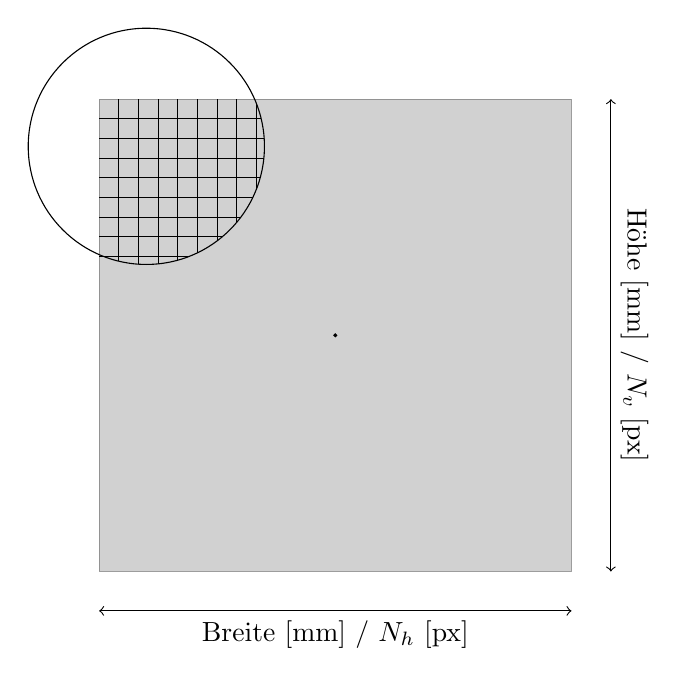
\begin{tikzpicture}
            \draw[fill=black!60!white,opacity=0.3] (-3, 3) -- (3, 3) -- (3, -3) -- (-3, -3) -- (-3, 3);
            \draw[fill=black] (0,0) circle (0.5pt);

            % Lupe
            \draw (-2.4, 2.4) circle (1.5cm);

            % Pixellinien vertikal
            \draw (-2.75, 3) -- (-2.75, 0.95);
            \draw (-2.5, 3) -- (-2.5, 0.9);
            \draw (-2.25, 3) -- (-2.25, 0.9);
            \draw (-2, 3) -- (-2, 0.95);
            \draw (-1.75, 3) -- (-1.75, 1.05);
            \draw (-1.5, 3) -- (-1.5, 1.2);
            \draw (-1.25, 3) -- (-1.25, 1.43);
            \draw (-1, 2.94) -- (-1, 1.85);

            % Pixellinien horizontal
            \draw (-3, 2.75) -- (-0.95, 2.75);
            \draw (-3, 2.5) -- (-0.9, 2.5);
            \draw (-3, 2.25) -- (-0.9, 2.25);
            \draw (-3, 2) -- (-0.95, 2);
            \draw (-3, 1.75) -- (-1.05, 1.75);
            \draw (-3, 1.5) -- (-1.2, 1.5);
            \draw (-3, 1.25) -- (-1.43, 1.25);
            \draw (-3, 1) -- (-1.85, 1);

            % Pfeile und Beschriftungen
            \draw[<->] (-3, -3.5) -- (3, -3.5) node[pos=0.5, below] {Breite [mm] / $N_h$ [px]};
            \draw[<->] (3.5, 3) -- (3.5, -3) node[pos=0.5, sloped, above] {Höhe [mm] / $N_v$ [px]};
        \end{tikzpicture}
        \captionof{figure}{Detektorgeometrie}
        \label{fig:det_geometrie}
    \end{minipage}%
    \begin{minipage}[b]{.5\textwidth}
        \centering
        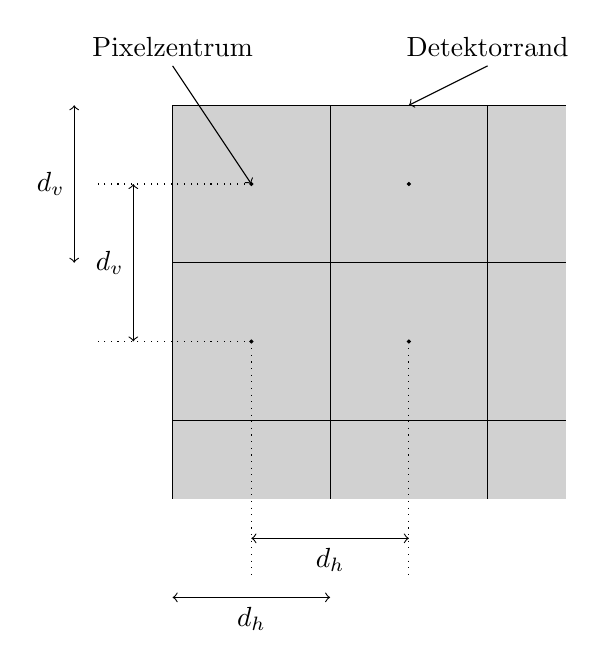
\begin{tikzpicture}
            \fill[black!60!white,opacity=0.3] (-2, 2) rectangle (3, -3);
            \draw (-2, 2) -- (2, 2) -- (2, -2) -- (-2, -2) -- (-2, 2);
            \draw (2, 2) -- (3, 2);
            \draw (-2, 0) -- (3, 0);
            \draw (0, 2) -- (0, -3);
            \draw (-2, 2) -- (-2, -3);
            \draw (2, -2) -- (2, -3);
            \draw (2, -2) -- (3, -2);
            \draw[fill=black] (-1, 1) circle (0.5pt);
            \draw[fill=black] (1, 1) circle (0.5pt);
            \draw[fill=black] (1, -1) circle (0.5pt);
            \draw[fill=black] (-1, -1) circle (0.5pt);

            % Verlängerungen
            \draw[dotted] (-1, 1) -- (-3, 1);
            \draw[dotted] (-1, -1) -- (-3, -1);
            \draw[dotted] (-1, -1) -- (-1, -4);
            \draw[dotted] (1, -1) -- (1, -4);

            % Pfeile und Beschriftungen
            \draw[->] (2, 2.5) -- (1, 2) node[pos=0, above] {Detektorrand};
            \draw[->] (-2, 2.5) -- (-1, 1) node[pos=0, above] {Pixelzentrum};
            \draw[<->] (-2.5, 1) -- (-2.5, -1) node[pos=0.5, left] {$d_v$};
            \draw[<->] (-3.25, 2) -- (-3.25, 0) node[pos=0.5, left] {$d_v$};
            \draw[<->] (-1, -3.5) -- (1, -3.5) node[pos=0.5, below] {$d_h$};
            \draw[<->] (-2, -4.25) -- (0, -4.25) node[pos=0.5, below] {$d_h$};
        \end{tikzpicture}
        \captionof{figure}{Pixelgeometrie}
        \label{fig:det_pixel}
    \end{minipage}
\end{figure}

\begin{figure}[!tb]
    \centering
    \begin{minipage}[b]{.5\textwidth}
        \centering
        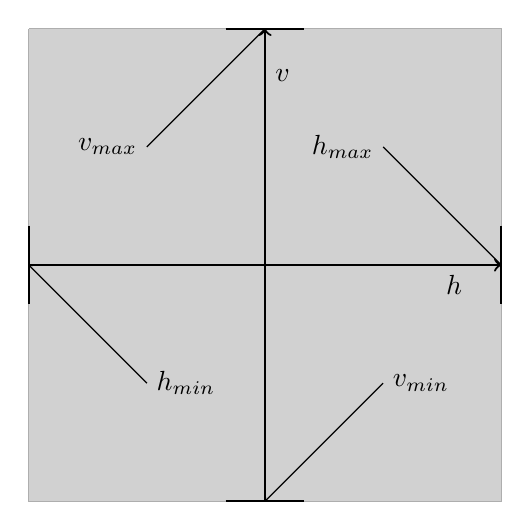
\begin{tikzpicture}[axis/.style={thick,->}]
            \draw[fill=black!60!white,opacity=0.3] (-3, 3) -- (3, 3) -- (3, -3) -- (-3, -3) -- (-3, 3);
            \draw[fill=black] (0,0) circle (0.5pt);

            % Achsen
            \draw[axis] (0, -3) -- (0, 3) node [pos=0.9, right] {$v$};
            \draw[axis] (-3, 0) -- (3, 0) node [pos=0.9, below] {$h$};

            % Markierungen
            \draw[thick] (-3, 0.5) -- (-3, -0.5);
            \draw[thick] (3, 0.5) -- (3, -0.5);
            \draw[thick] (-0.5, 3) -- (0.5, 3);
            \draw[thick] (-0.5, -3) -- (0.5, -3);

            % Beschriftungen
            \draw[->] (1.5, 1.5) -- (3, 0) node [pos=0, left] {$h_{max}$};
            \draw[->] (-1.5, -1.5) -- (-3, 0) node [pos=0, right] {$h_{min}$};
            \draw[->] (-1.5, 1.5) -- (0, 3) node [pos=0, left] {$v_{max}$};
            \draw[->] (1.5, -1.5) -- (0, -3) node [pos=0, right] {$v_{min}$};
        \end{tikzpicture}
        \caption{Detektorkoordinatensystem}
        \label{fig:det_koord}
    \end{minipage}%
    \begin{minipage}[b]{.5\textwidth}
        \centering
        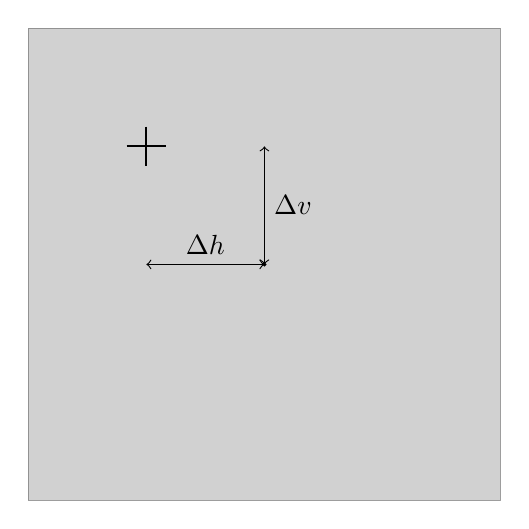
\begin{tikzpicture}
            \draw[fill=black!60!white,opacity=0.3] (-3, 3) -- (3, 3) -- (3, -3) -- (-3, -3) -- (-3, 3);
            \draw[fill=black] (0,0) circle (0.5pt);

            % Verschiebung
            \draw[thick] (-1.75, 1.5) -- (-1.25, 1.5);
            \draw[thick] (-1.5, 1.75) -- (-1.5, 1.25);

            % Pfeile & Beschriftung
            \draw[<->] (0, 1.5) -- (0, 0) node[pos=0.5,right] {$\Delta v$};
            \draw[<->] (0, 0) -- (-1.5, 0) node[pos=0.5,above] {$\Delta h$};
        \end{tikzpicture}
        \caption{Verschiebungsgeometrie}
        \label{fig:off_geometrie}
    \end{minipage}
\end{figure}

\subsubsection{Verschiebungen}

In einem idealen Modell sind die Strahlungsquelle und der Detektor genau aufeinander ausgerichtet, das heißt, dass der
Mittelpunkt der Strahlungsquelle und der Mittelpunkt des Detektors auf derselben Achse liegen. Durch den mechanischen
Aufbau einer realen Computertomographie-Anlage und deren händischer Justierung kommt es allerdings zu sowohl
einer horizontalen Verschiebung $\Delta h$ als auch einer vertikalen Verschiebung $\Delta v$ dieser Achse (siehe
Abbildung~\ref{fig:off_geometrie}). Von der Strahlungsquelle ausgehend trifft sie somit nicht mehr auf das Zentrum des
Detektors, sondern auf einen anderen Teil. Nimmt man Bezug auf die Detektorgeometrie, so müssen diese Verschiebungen
entsprechend berücksichtigt werden, da ansonsten ein verfälschtes Ergebnis berechnet wird. Dazu müssen die
Formeln~\ref{eq:det_h} und~\ref{eq:det_v} wie folgt umgeschrieben werden:

\begin{equation} 
    h_{min} + \frac{N_h \cdot d_h}{2} + \Delta h = 0
\end{equation}

\begin{equation}
    v_{min} + \frac{N_v \cdot d_v}{2}  + \Delta v = 0
\end{equation}

\subsubsection{Fehlende Projektionen}

Es leuchtet ein, dass Projektionen, die im Abstand von 180° aufgenommen wurden, das durchleuchtete Objekt
spiegelverkehrt darstellen. In der Theorie würde es also ausreichen, einen Halbkreis um das Objekt abzufahren, um alle
erforderlichen Informationen für die Rückprojektion zu gewinnen. In der Praxis kann es aufgrund mechanischer Fehler bei
der Rotation des Quelle-Detektor-Aufbaus allerdings dazu kommen, dass einzelne Projektionen übersprungen werden oder die
Winkelabstände zwischen zwei Projektionen verschieden groß sind. Das Abfahren eines Vollkreises dient dazu, die so
entstandenen Fehler durch Redundanzen zu minimieren.

\subsection{Geometrische Berechnungen}

\begin{itemize}
    \item Berechnung der Volumengeometrie
    \item Aufteilung in Teilvolumen
\end{itemize}

\subsection{Implementierung der Vorstufen}

\subsubsection{Wichtung}

Die Grundlage der Wichtungsoperation ist die in Abschnitt~\ref{sssec:fdk_wichtung} vorgestellte
Formel~\ref{eq:wichtung}:

\begin{equation*}
    w_{ij} = \frac{d_{det} - d_{src}}{\sqrt{(d_{det} - d_{src})^2 + h_j^2 + v_i^2}}
\end{equation*}

Es ist leicht zu sehen, dass sich der Wichtungsfaktor $w_{ij}$ zwar pro \gls{pixel} ändert, aber nicht von der konkreten
Projektion abhängig ist. Es ist daher möglich, die Berechnung der Wichtungsfaktoren am Anfang des Programms genau einmal
durchzuführen und in einer Wichtungsmatrix \texttt{m} zu speichern (siehe Quelltext~\ref{source:impl_gen_mat}). Die
Berechnung der Wichtungsmatrix hängt von mehreren geometrischen Parametern ab (vgl.\
Abschnitt~\ref{sssec:fdk_geometrie} und Abbildungen~\ref{fig:det_geometrie},~\ref{fig:det_pixel},~\ref{fig:det_koord},~\ref{fig:off_geometrie}):

\begin{itemize}
    \item \texttt{dim\_x}: Anzahl der \gls{pixel} in horizontaler Richtung. Entspricht der Anzahl der Detektorpixel in
          horizontaler Richtung $N_h$
    \item \texttt{dim\_y}: Anzahl der \gls{pixel} in vertikaler Richtung. Entspricht der Anzahl der Detektorpixel in
          vertikaler Richtung $N_v$
    \item \texttt{h\_min}: horizontaler Abstand vom Detektorrand zum Detektorzentrum in mm.
    \item \texttt{v\_min}: vertikaler Abstand vom Detektorrand zum Detektorzentrum in mm.
    \item \texttt{d\_sd}: Abstand von der Quelle zum Detektor. Entsprich der Differenz der Strecken $d_{det}$ (Abstand
          zwischen dem Objekt und dem Detektor) und $d_{src}$ (Abstand zwischen der Quelle und dem Objekt) bzw.\ der
          Summe ihrer Beträge:
          
          \begin{equation*}
              d_{det} - d_{src} = |d_{det}| + |d_{src}|
          \end{equation*}

    \item \texttt{l\_px\_row}: horizontale Länge eines \gls{pixel}s, also der horizontale Abstand zwischen den
          Mittelpunkten zweier aufeinanderfolgender \gls{pixel}. Entspricht der horizontalen Länge eines Detektorpixels
          $d_h$.
    \item \texttt{l\_px\_col}: vertikale Länge eines \gls{pixel}s, also der vertikale Abstand zwischen den
          Mittelpunkten zweier aufeinanderfolgender \gls{pixel}. Entspricht der vertikalen Länge eines Detektorpixels
          $d_v$.
\end{itemize}

\begin{code}
\begin{minted}[breaklines,breakafter=\,,fontsize=\small]{cuda}
__global__ void matrix_generation_kernel(float* m,
    std::uint32_t dim_x, std::uint32_t dim_y, std::size_t pitch,
    float h_min, float v_min, float d_sd, float l_px_row,
    float l_px_col)
{
    auto s = blockIdx.x * blockDim.x + threadIdx.x;
    auto t = blockIdx.y * blockDim.y + threadIdx.y;

    if((s < dim_x) && (t < dim_y))
    {
        auto row = reinterpret_cast<float*>(
            reinterpret_cast<char*>(m) + t * pitch);

        // Detektorkoordinaten in mm
        const auto h_s = (l_px_row / 2.f) + s * l_px_row + h_min;
        const auto v_t = (l_px_col / 2.f) + t * l_px_col + v_min;

        // berechne Wichtungsfaktor
        row[s] = d_sd * rsqrtf(d_sd * d_sd + h_s * h_s + v_t * v_t);
    }
}
\end{minted}
\captionof{listing}{Generierung der Wichtungsmatrix}
\label{source:impl_gen_mat}
\end{code}

Bei der Wichtung einer Projektion \texttt{p} kann der jeweilige Wichtungsfaktor aus der generierten Matrix \texttt{m}
ausgelesen und auf das zugehörige \gls{pixel} angewendet werden (siehe Quelltext~\ref{source:impl_weighting}). Die so
gewichtete Projektion wird dann im folgenden Schritt gefiltert.

\begin{code}
\begin{minted}[breaklines,breakafter=\,,escapeinside=||,fontsize=\small]{cuda}
__global__ void weighting_kernel(float* p, const float* m,
    std::uint32_t dim_x, std::uint32_t dim_y, std::size_t pitch,
    std::size_t m_pitch)
{
    auto s = blockIdx.x * blockDim.x + threadIdx.x;
    auto t = blockIdx.y * blockDim.y + threadIdx.y;

    if((s < dim_x) && (t < dim_y))
    {
        auto p_row = |\textbf{\textcolor{keyword-green}{reinterpret\_cast}}|<float*>(
            |\textbf{\textcolor{keyword-green}{reinterpret\_cast}}|<char*>(p) + t * pitch);
        auto m_row = |\textbf{\textcolor{keyword-green}{reinterpret\_cast}}|<const float*>(
            |\textbf{\textcolor{keyword-green}{reinterpret\_cast}}|<const char*>(m) + t * m_pitch);

        // Wichtung
        p_row[s] *= m_row[s];
    }
}
\end{minted}
\captionof{listing}{Wichtung einer Projektion}
\label{source:impl_weighting}
\end{code}

\subsubsection{Filterung}

Dem in Abschnitt~\ref{sssec:fdk_filter} vorgestellten Algorithmus entsprechend, folgt die Implementierung des
Filterschrittes dem nachstehenden Schema:

\begin{enumerate}
    \item einmalige Erzeugung und Fouriertransformation des Filters
    \item zeilenweise Fouriertransformation der Projektion
    \item Anwendung des Filters auf die jeweilige Projektionszeile im komplexen Raum
    \item inverse zeilenweise Fouriertransformation der Projektion
\end{enumerate}

Die Implementierung der Filtergenerierung entspricht der Formel~\ref{eq:filter_gen} und kann dem im Anhang befindlichen
Quelltext~\ref{app:filter_gen} entnommen werden. Dieser Filter wird dann zeilenweise auf jede Projektion angewendet.
Dazu werden der Filter und die einzelnen Projektionszeilen mit der \gls{cufft}-Bibliothek zunächst fouriertransformiert.
Im komplexen Raum werden dann die einzelnen Elemente der transformierten Projektionszeile mit den korrespondierenden
Elementen des transformierten Filters multipliziert (siehe Quelltext~\ref{source:impl_filter}). Ist dieser Vorgang
abgeschlossen, wird die Projektion wieder zurücktransformiert und normalisiert (siehe den angehängten
Quelltext~\ref{app:filter_norm}). Die Projektion ist dann bereit für die Rückprojektion.

\begin{code}
\begin{minted}[breaklines,breakafter=\,,fontsize=\small]{cuda}
__global__ void filter_application_kernel(
    cufftComplex* __restrict__ data,
    const cufftComplex* __restrict__ filter,
    std::uint32_t filter_size, std::uint32_t data_height,
    std::size_t pitch)
{
    auto x = blockIdx.x * blockDim.x + threadIdx.x;
    auto y = blockIdx.y * blockDim.y + threadIdx.y;

    if((x < filter_size) && (y < data_height))
    {
        auto row = reinterpret_cast<cufftComplex*>(
            reinterpret_cast<char*>(data) + y * pitch);

        row[x].x *= filter[x].x;
        row[x].y *= filter[x].y;
    }
}
\end{minted}
\captionof{listing}{Filterung einer Projektion}
\label{source:impl_filter}
\end{code}

\subsection{Implementierung der gefilterten Rückprojektion}

\begin{itemize}
    \item welche Konstanten und Variablen gibt es
    \item welche Schwierigkeiten können auftreten
\end{itemize}

\chapter{Ergebnisse und Diskussion}

\section{Leistungsmessung}

\subsection{Gesamtprogramm}

Messungen des Gesamtprogramms (Datentransfers, alle Stufen)

\subsection{Teilstufen}

grobe Messungen der Teilstufen (Wichtung, Filterung, Rückprojektion)

Ergebnis: Rückprojektion braucht am längsten

\subsection{Eigenschaften des Rückprojektionskernels}

In Abschnitt~\ref{ssec:opti_ueber} wurde als Implementierungsziel unter anderem eine möglichst hohe \gls{gpu}-Auslastung
gefordert. Um diese Auslastung zu erreichen, ist ein möglichst geringer Verbrauch der zwischen den Threads geteilten
Ressourcen erforderlich. Da der \textit{Shared Memory} in der Implementierung nicht verwendet wurde, zielte die
Umsetzung dieser Forderung auf einen möglichst geringen Registerverbrauch ab.

Wie in Abbildung~\ref{fig:kernel_props} zu sehen ist, benötigt der Rückprojektions-\gls{kernel} 19 Register
(grün markiert). Auf der hier verwendeten GeForce GTX 1080 ist somit eine theoretische Auslastung der gesamten \gls{gpu}
möglich, praktisch wird die \gls{gpu} durch die Rückprojektion zu 88,5\% ausgelastet (rot markiert).

Ein weiteres der drei Optimierungsziele, die in Abschnitt~\ref{ssec:opti_ueber} genannt wurden, ist die Verkürzung der
Wartezeit zwischen dem Ende einer Rückprojektion und dem Beginn der nachfolgenden Rückprojektion. Zu diesem Zweck wird
die Rückprojektion in einem eigenen Thread und \gls{cuda}-Stream ausgeführt, sodass die vorherigen Operationen (Laden,
Wichten, Filtern) parallel zur Rückprojektion ausgeführt werden können. Der Rückprojektionsthread entnimmt die nächste
Projektion vom Stapel der noch ausstehenden Projektionen, wandelt diese in eine \gls{cuda}-Textur um und startet dann
den Rückprojektions-\gls{kernel}. Wie Abbildung~\ref{fig:kernel_wait} zeigt, ist es gelungen, die Zeit zwischen zwei
Rückprojektionen, die durch die langen, grün-blauen Balken dargestellt werden, auf 2 Millisekunden zu beschränken. Bei
einem üblichen Datensatz von 1440 Projektionen ergibt sich also eine Gesamtwartezeit von 2,88 Sekunden.

Abbildung~\ref{fig:kernel_wait} zeigt allerdings auch, dass diese Wartezeit noch nicht ideal ist. Das Ziel, die Wichtung
und die Filterung, die durch die kleineren, bunten Balken repräsentiert werden, parallel zur Rückprojektion
durchzuführen, konnte nicht erreicht werden. Der Grund dafür ist vermutlich die Anzahl der Threads, die vom
Rückprojektions-\gls{kernel} gestartet werden. Bei einem Volumen mit 1070 x 1070 x 1033 \gls{voxel}n, denen jeweils ein
Thread zugeordnet wird, werden 1.182.681.700 Threads benötigt. Die GTX 1080 verfügt über 20 \gls{sm}s, von denen jeder
bis zu 2.048 Threads gleichzeitig ausführen kann und kann somit bis zu 40.960 Threads gleichzeitig verwalten. Die
\gls{gpu} ist daher gezwungen, der Rückprojektion alle verfügbaren Threads zuzuweisen, was zur Folge hat, dass keine
weiteren \gls{kernel} ausgeführt werden können. Wenn auch die parallele Ausführung der Rückprojektion und der vorherigen
Schritte nicht gelungen ist, ist auf der Abbildung jedoch zu sehen, dass die Ausführung der \gls{kernel} mit geringerem
Ressourcenbedarf sich stellenweise überlappt.

Die Wartezeit zwischen zwei Rückprojektionen, die über die gesamte Laufzeit akkumuliert ca. 3 Sekunden einnimmt, hat
also einen akzeptablen Wert erreicht, der dem alltäglichen Gebrauch nicht im Wege steht. Auch wenn an dieser Stelle noch
Optimierungspotential vorhanden ist, wäre selbst eine vollständige Eliminierung der Wartezeit vernachlässigbar.

\begin{figure}
    \includegraphics[width=\linewidth]{img/kernel_properties}
    \caption{Eigenschaften des Rückprojektionskernels}
    \label{fig:kernel_props}
\end{figure}

\begin{figure}
    \includegraphics[width=\linewidth]{img/timeline_compute3}
    \caption{Zeit zwischen zwei Rückprojektionen}
    \label{fig:kernel_wait}
\end{figure}

\subsection{Laufzeitverhalten}

Die parallele Berechnung verschiedener Teile des Volumens durch den Einsatz mehrerer \gls{gpu}s war ebenfalls ein
Implementierungsziel. Die besondere Herausforderung bestand darin, sowohl mehrere \gls{gpu}s des gleichen Typs als auch
unterschiedliche \gls{gpu}s zu unterstützen.

Wie Abbildung~\ref{fig:kernel_multi_compute} zeigt, ist es gelungen, die Ausführung parallel auf mehreren \gls{gpu}s
durchzuführen. Der gewählte Ansatz zur Lastverteilung (siehe Abschnitt~\ref{}) führt jedoch bei unterschiedlich
leistungsstarken \gls{gpu}s dazu, dass die stärkere \gls{gpu} vor der schwächeren fertig ist und dann auf diese warten
muss, wie in Abbildung~\ref{fig:kernel_multi_bad} zu sehen ist.

In Abbildung~\ref{fig:laufzeit_gpus} ist das Laufzeitverhalten unterschiedlicher \gls{gpu}s dargestellt. Es ist klar
zu sehen, dass der gemeinsame Einsatz der Tesla K20c und der GTX 1080 in diesem Fall sogar zu einer längeren Laufzeit
führt, als der alleinige Einsatz der GTX 1080. Die statische Lastverteilung, wie sie in dieser Arbeit beschrieben ist,
sollte daher zukünftig auf heterogenen \gls{gpu}-Systemen durch andere Methoden abgelöst werden. Denkbar ist
beispielsweise der Einsatz von \textit{Machine-Learning}-Techniken, durch die die optimale Lastverteilung iterativ
ermittelt wird.

\begin{figure}
    \includegraphics[width=\linewidth]{img/timeline_multi_compute}
    \caption{Parallele Ausführung auf zwei \gls{gpu}s}
    \label{fig:kernel_multi_compute}
\end{figure}

\begin{figure}
    \includegraphics[width=\linewidth]{img/timeline_multi_bad}
    \caption{Der gewählte, statische Lastverteilungsansatz führt zu Wartezeiten}
    \label{fig:kernel_multi_bad}
\end{figure}

\begin{figure}
    \centering
    \begin{tikzpicture}
        \begin{axis}[width=\textwidth,
                     xlabel={Volumengröße [Voxel]},
                     symbolic x coords={133 x 133 x 129,267 x 267 x 258,535 x 535 x 516, 1070 x 1070 x 1033},
                     xtick=data,
                     ylabel={Laufzeit [s]},
                     legend pos=north west]

             \addplot table[x=Volumengroesse,y=GTX1080,col sep=comma] {data/mehreregpus.csv};
             \addplot table[x=Volumengroesse,y=K20c,col sep=comma] {data/mehreregpus.csv};
             \addplot table[x=Volumengroesse,y=GTX1080K20c,col sep=comma] {data/mehreregpus.csv};
             \legend{GTX 1080,Tesla K20c,GTX \& Tesla};
        \end{axis}
    \end{tikzpicture}
    \caption{Laufzeit mit mehreren \gls{gpu}s}
    \label{fig:laufzeit_gpus}
\end{figure}

\section{Vergleich mit der Literatur}

Der Vergleich mit den oben vorgestellten Ansätzen der Literatur ist ebenfalls von Interesse. Da Zhao et al.\ in ihrer
Arbeit nur Zeiten für die Rückprojektion angeben, werden im Vergleich mit der von ihnen vorgestellten Variante ebenfalls
nur die Zeiten der Rückprojektion berücksichtigt. Scherl et al.\ beziehen dagegen auch die Datenein- und -ausgabe mit
ein. Zur Messung wurde von Zhao et al.\ die 2007 erschienene NVIDIA Quadro FX4600 eingesetzt, die über 768 MiB Speicher
verfügt; Scherl et al.\ verwendeten die 2006 vorgestellte NVIDIA GeForce 8800 GTX, die ebenfalls mit 768 MiB Speicher
ausgerüstet ist. Für den Vergleich fand in dieser Arbeit die 2016 präsentierte NVIDIA GeForce GTX 1080 Verwendung, die
mit 8 GiB Speicher ausgestattet ist.

Wie die obere Hälfte der Tabelle~\ref{table:paris_vs_scherl_zhao} zeigt, kann die vorgestellte Implementierung die von
Scherl et al.\ erreichten Werte, inklusive der Datenein- und Ausgabe, auf modernerer Hardware um ein Viertel
unterbieten. Es ist ebenfalls gelungen, die von Zhao et al.\ vorgestellten Zeitangaben auf bis zu ein Drittel der Zeit
zu reduzieren.

\begin{table}
    \centering
    \begin{tabular}{llccc}
        \hline
        & GPU & Volumengröße [Voxel] & Projektionszahl & Zeitbedarf [s]\\
        \hline
        Scherl et al. & GeForce 8800 GTX & 512 x 512 x 512 & 414 & 12\\
        Stephan & GeForce GTX 1080 & 512 x 512 x 512 & 360 & 9\\
        Stephan & GeForce GTX 1080 & 512 x 512 x 512 & 480 & 9\\
        \hline
        Zhao et al. & Quadro FX4600 & 512 x 512 x 512 & 360 & 7,7\\
        Stephan & GeForce GTX 1080 & 512 x 512 x 512 & 360 & 2\\
        Zhao et al. & Quadro FX4600 & 1024 x 1024 x 1024 & 720 & 101,9\\
        Stephan & GeForce GTX 1080 & 1024 x 1024 x 1024 & 720 & 34\\
        \hline
    \end{tabular}
    \caption{Vergleich mit denen von Scherl et al.\ und Zhao et al.\ vorgestellten Ansätzen}
    \label{table:paris_vs_scherl_zhao}
\end{table}

\chapter{Zusammenfassung und Ausblick}

Es wurde in dieser Arbeit eine mögliche Implementierung des \gls{fdk} auf dem Fundament der CUDA-Plattform vorgestellt.
Das Ziel, die Rückprojektion in sinnvoller Zeit zu berechnen, ist erreicht worden. Abhängig von der gewünschten Größe
des Volumens benötigt der Algorithmus auf moderner Hardware wenige Sekunden bis Minuten. Die Wartezeit zwischen zwei
Rückprojektionen konnte auf wenige Millisekunden reduziert werden. Insbesondere bei großen Volumen ist sie dadurch
vernachlässigbar gering, da sie, akkumuliert über die gesamte Laufzeit von einigen Minuten, lediglich wenige Sekunden
einnimmt. Bei der Rekonstruktion kleinerer Volumen fällt sie allerdings stärker ins Gewicht.

Es wurde ebenfalls erreicht, dass der Rückprojektions-\gls{kernel} die \gls{gpu} möglichst stark auslastet. Außerdem
gelang es, den Algorithmus so zu implementieren, dass er bei der Berechnung großer Volumen von mehreren \gls{gpu}s des
gleichen Typs beschleunigt wird. Die Rekonstruktion kleinerer Volumen profitiert allerdings nicht vom Einsatz mehrerer
Grafikkarten; eine einzelne \gls{gpu} war in allen Fällen schneller. Die Verwendung verschiedener \gls{gpu}s kann
außerdem dazu führen, dass der Algorithmus langsamer ausgeführt wird, als wenn man nur die leistungsstärkere Grafikkarte
verwendet hätte.

Die Verwendung von CUDA hat sich für die Parallelisierung des \gls{fdk} als vorteilhaft erwiesen. Durch die massiv
datenparallele Philosophie eignet sich CUDA gut für die Berechnung unabhängiger \gls{voxel}. Aufgrund der
Spezialisierung der \gls{gpu}s auf grafische Operationen sind sie gut für den Einsatz in bildgebenden Messverfahren wie
der Computertomographie geeignet. Eine Hürde, die beachtet werden muss, bleibt allerdings der begrenzte Speicher,
besonders im Hinblick auf die von neuen und zukünftigen Computertomographieanlagen erzeugten Datenmengen.

Wie die Analyse gezeigt hat, ist die vorgestellte Implementierung noch nicht an allen Stellen optimal. Insbesondere ist
es bei kleinen Volumen nicht gelungen, die in der Literatur präsentierten Zeiten für die Rekonstruktion zu erreichen,
was vermutlich auf zu starken Host-Overhead zurückzuführen ist. Dieser Overhead steigt durch den Einsatz mehrerer
\gls{gpu}s sogar noch weiter an, sodass der nächste Optimierungsschritt des Programms darin bestehen muss, die
Operationen auf der \gls{host}-Seite zu optimieren.

Die Skalierung des \gls{fdk} über mehrere \gls{gpu}s ist insgesamt verbesserungswürdig. Die Tatsache, dass selbst bei
der Rekonstruktion großer Volumen der Einsatz zwei verschiedener \gls{gpu}s länger dauert als der alleinige Einsatz der
leistungsstärkeren Karte, zeigt deutlich die Limitierungen der verwendeten statischen Lastverteilung. Denkbar ist hier
eine vor der Rückprojektion stattfindende algorithmische Bestimmung der idealen Last pro \gls{gpu}, beispielsweise in
Abhängigkeit von der Taktfrequenz und dem verfügbaren Speicher der jeweiligen Grafikkarte. Auch der Einsatz von
\textit{Machine-Learning}-Techniken kann in Betracht gezogen werden.

Die gefilterte Rückprojektion könnte außerdem durch einige Ansätze aus der Literatur weiter verbessert werden. Bei
großen Volumen wäre die Ausnutzung der Symmetrien, wie sie von Zhao et al.\ vorgeschlagen wird, eine Möglichkeit zur
weiteren Geschwindigkeitssteigerung. Der Ansatz von Scherl et al.\, mit einem zweidimensionalen Kernel durch das Volumen
zu iterieren, könnte die Zahl der für die Rückprojektion benötigten Ressourcen reduzieren und so auf dem \gls{device}
die zur Rückprojektion parallele Ausführung der Wichtung und Filterung erlauben. Dadurch wäre es möglich, die Zeit
zwischen zwei Rückprojektionen weiter zu reduzieren.

Die vorgestellte Implementierung des \gls{fdk} berechnet die Rückprojektion für derzeit gängige Projektionsdatensätze
in wenigen Minuten. Aufgrund der Aufnahmegeschwindigkeit einer Computertomographieanlage ist es denkbar, die
generierten Projektionen in Echtzeit zu verarbeiten. Die für die Berechnung benötigte Zeit könnte so durch die Aufnahme
verdeckt werden, sodass am Ende der Aufnahme bereits ein rekonstruiertes Volumen vorliegt. Dabei wäre es möglich bzw.\
für die Echtzeitrekonstruktion notwendig, vor der Wichtung und der Filterung der Projektionen zusätzliche
Vorverarbeitungsschritte in den Algorithmus zu integrieren, wie etwa eine Korrektur defekter Pixel oder eine
automatische Berücksichtigung des Detektor-Offsets.

Das im Rahmen dieser Arbeit am Helmholtz-Zentrum Dresden-Rossendorf entstandene Programm wurde unter eine freie Lizenz
gestellt. Der Quelltext ist im Internet unter der nachstehenden Adresse verfügbar:
\url{https://www.github.com/HZDR-FWDF/PARIS}


\end{document}
